%4
\section{Konkrete Architektur}

Abbildung \ref{KomponentendiagrammKonkret} zeigt die Komponenten \emph{ServerSoftware} und \emph{RobotSoftware} sowie deren Zusammenhang in einem Komponentendiagramm. \\ Die Kommunikation der Komponenten findet abstrahiert über \emph{Remote Procedure Calls} (RPC) statt, sodass der \emph{Server} auf der \emph{RobotUnit} die in den Schnittstellen \emph{ISensorData} und \emph{ITask} definierten Methoden wie lokale Aufrufe ausführen kann. Umgekehrt kann die \emph{RobotUnit} über die Schnittstellen \emph{IRepair} und \emph{IArrivalNotification} Methoden auf dem \emph{Server} aufrufen.

\begin{figure}[H]
\centering
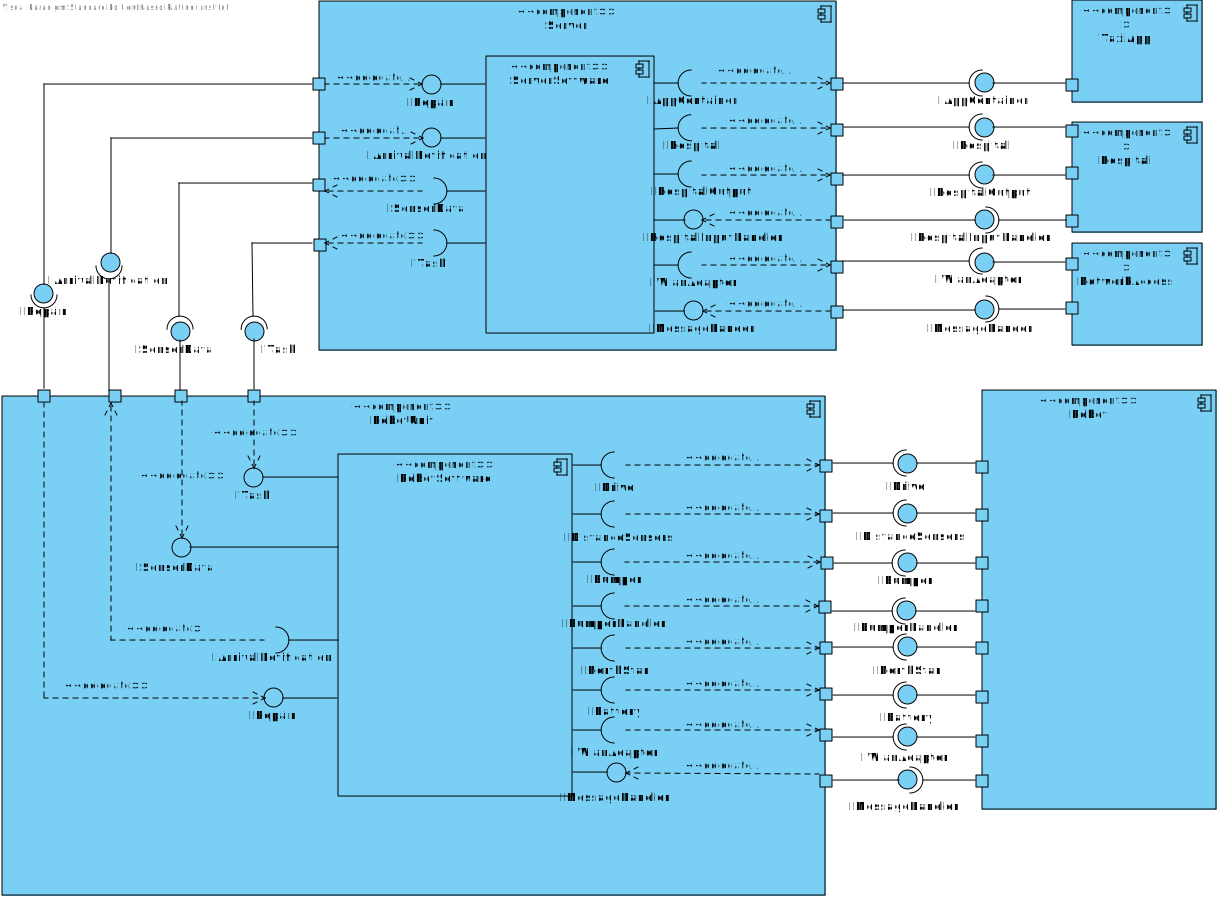
\includegraphics[width=1\textwidth]{img/2-Entwurf-4-KonkreteArchitektur}
\caption{Komponentendiagramm mit den Komponentenschnittstellen}
\label{KomponentendiagrammKonkret}
\end{figure}

%4.1 Server Software
\subsection{\textit{ServerSoftware}}
%- Externe Kommunikation: - Entgegennahme von Aufträgen, Mitteilung über Auftragsabarbeitung, etc.
%- Interne Kommunikation: - Taskdistribution
%- Verwaltung der Tasks
%- 

Die auf dem \emph{Server} laufende \emph{ServerSoftware} koordiniert sowohl die externe als auch die interne Kommunikation und übernimmt sämtliche Verwaltungsaufgaben.
Sie nimmt von extern an das System gestellte \emph{Orders} entgegen und verteilt sie mittels einer \emph{PriorityQueue} an die verfügbaren \emph{RobotUnits}. Im Verlauf der Abarbeitung einer \emph{Task} kommuniziert die \emph{ServerSoftware} mit dem Auftraggeber.

%4.2 Robot Software
\subsection{\textit{RobotSoftware}}

\emph{RobotSoftware} ist für die Steuerung der \textit{RobotUnit} zuständig. 
Die von der abstrakten Hardware
des \textit{Robot} angebotenen, vorgegebenen Interfaces \textit{INorthStar, IBattery, IDrive, IDistanceSensors, IBumper} sowie
\textit{IBumperHandler} werden dabei von der \textit{Robot}-Komponente für die konkrete Steuerung der \textit{RobotUnit} genutzt.
